% Options for packages loaded elsewhere
\PassOptionsToPackage{unicode}{hyperref}
\PassOptionsToPackage{hyphens}{url}
\PassOptionsToPackage{dvipsnames,svgnames,x11names}{xcolor}
%
\documentclass[
  letterpaper,
  DIV=11,
  numbers=noendperiod]{scrartcl}

\usepackage{amsmath,amssymb}
\usepackage{lmodern}
\usepackage{iftex}
\ifPDFTeX
  \usepackage[T1]{fontenc}
  \usepackage[utf8]{inputenc}
  \usepackage{textcomp} % provide euro and other symbols
\else % if luatex or xetex
  \usepackage{unicode-math}
  \defaultfontfeatures{Scale=MatchLowercase}
  \defaultfontfeatures[\rmfamily]{Ligatures=TeX,Scale=1}
\fi
% Use upquote if available, for straight quotes in verbatim environments
\IfFileExists{upquote.sty}{\usepackage{upquote}}{}
\IfFileExists{microtype.sty}{% use microtype if available
  \usepackage[]{microtype}
  \UseMicrotypeSet[protrusion]{basicmath} % disable protrusion for tt fonts
}{}
\makeatletter
\@ifundefined{KOMAClassName}{% if non-KOMA class
  \IfFileExists{parskip.sty}{%
    \usepackage{parskip}
  }{% else
    \setlength{\parindent}{0pt}
    \setlength{\parskip}{6pt plus 2pt minus 1pt}}
}{% if KOMA class
  \KOMAoptions{parskip=half}}
\makeatother
\usepackage{xcolor}
\setlength{\emergencystretch}{3em} % prevent overfull lines
\setcounter{secnumdepth}{-\maxdimen} % remove section numbering
% Make \paragraph and \subparagraph free-standing
\ifx\paragraph\undefined\else
  \let\oldparagraph\paragraph
  \renewcommand{\paragraph}[1]{\oldparagraph{#1}\mbox{}}
\fi
\ifx\subparagraph\undefined\else
  \let\oldsubparagraph\subparagraph
  \renewcommand{\subparagraph}[1]{\oldsubparagraph{#1}\mbox{}}
\fi

\usepackage{color}
\usepackage{fancyvrb}
\newcommand{\VerbBar}{|}
\newcommand{\VERB}{\Verb[commandchars=\\\{\}]}
\DefineVerbatimEnvironment{Highlighting}{Verbatim}{commandchars=\\\{\}}
% Add ',fontsize=\small' for more characters per line
\usepackage{framed}
\definecolor{shadecolor}{RGB}{241,243,245}
\newenvironment{Shaded}{\begin{snugshade}}{\end{snugshade}}
\newcommand{\AlertTok}[1]{\textcolor[rgb]{0.68,0.00,0.00}{#1}}
\newcommand{\AnnotationTok}[1]{\textcolor[rgb]{0.37,0.37,0.37}{#1}}
\newcommand{\AttributeTok}[1]{\textcolor[rgb]{0.40,0.45,0.13}{#1}}
\newcommand{\BaseNTok}[1]{\textcolor[rgb]{0.68,0.00,0.00}{#1}}
\newcommand{\BuiltInTok}[1]{\textcolor[rgb]{0.00,0.23,0.31}{#1}}
\newcommand{\CharTok}[1]{\textcolor[rgb]{0.13,0.47,0.30}{#1}}
\newcommand{\CommentTok}[1]{\textcolor[rgb]{0.37,0.37,0.37}{#1}}
\newcommand{\CommentVarTok}[1]{\textcolor[rgb]{0.37,0.37,0.37}{\textit{#1}}}
\newcommand{\ConstantTok}[1]{\textcolor[rgb]{0.56,0.35,0.01}{#1}}
\newcommand{\ControlFlowTok}[1]{\textcolor[rgb]{0.00,0.23,0.31}{#1}}
\newcommand{\DataTypeTok}[1]{\textcolor[rgb]{0.68,0.00,0.00}{#1}}
\newcommand{\DecValTok}[1]{\textcolor[rgb]{0.68,0.00,0.00}{#1}}
\newcommand{\DocumentationTok}[1]{\textcolor[rgb]{0.37,0.37,0.37}{\textit{#1}}}
\newcommand{\ErrorTok}[1]{\textcolor[rgb]{0.68,0.00,0.00}{#1}}
\newcommand{\ExtensionTok}[1]{\textcolor[rgb]{0.00,0.23,0.31}{#1}}
\newcommand{\FloatTok}[1]{\textcolor[rgb]{0.68,0.00,0.00}{#1}}
\newcommand{\FunctionTok}[1]{\textcolor[rgb]{0.28,0.35,0.67}{#1}}
\newcommand{\ImportTok}[1]{\textcolor[rgb]{0.00,0.46,0.62}{#1}}
\newcommand{\InformationTok}[1]{\textcolor[rgb]{0.37,0.37,0.37}{#1}}
\newcommand{\KeywordTok}[1]{\textcolor[rgb]{0.00,0.23,0.31}{#1}}
\newcommand{\NormalTok}[1]{\textcolor[rgb]{0.00,0.23,0.31}{#1}}
\newcommand{\OperatorTok}[1]{\textcolor[rgb]{0.37,0.37,0.37}{#1}}
\newcommand{\OtherTok}[1]{\textcolor[rgb]{0.00,0.23,0.31}{#1}}
\newcommand{\PreprocessorTok}[1]{\textcolor[rgb]{0.68,0.00,0.00}{#1}}
\newcommand{\RegionMarkerTok}[1]{\textcolor[rgb]{0.00,0.23,0.31}{#1}}
\newcommand{\SpecialCharTok}[1]{\textcolor[rgb]{0.37,0.37,0.37}{#1}}
\newcommand{\SpecialStringTok}[1]{\textcolor[rgb]{0.13,0.47,0.30}{#1}}
\newcommand{\StringTok}[1]{\textcolor[rgb]{0.13,0.47,0.30}{#1}}
\newcommand{\VariableTok}[1]{\textcolor[rgb]{0.07,0.07,0.07}{#1}}
\newcommand{\VerbatimStringTok}[1]{\textcolor[rgb]{0.13,0.47,0.30}{#1}}
\newcommand{\WarningTok}[1]{\textcolor[rgb]{0.37,0.37,0.37}{\textit{#1}}}

\providecommand{\tightlist}{%
  \setlength{\itemsep}{0pt}\setlength{\parskip}{0pt}}\usepackage{longtable,booktabs,array}
\usepackage{calc} % for calculating minipage widths
% Correct order of tables after \paragraph or \subparagraph
\usepackage{etoolbox}
\makeatletter
\patchcmd\longtable{\par}{\if@noskipsec\mbox{}\fi\par}{}{}
\makeatother
% Allow footnotes in longtable head/foot
\IfFileExists{footnotehyper.sty}{\usepackage{footnotehyper}}{\usepackage{footnote}}
\makesavenoteenv{longtable}
\usepackage{graphicx}
\makeatletter
\def\maxwidth{\ifdim\Gin@nat@width>\linewidth\linewidth\else\Gin@nat@width\fi}
\def\maxheight{\ifdim\Gin@nat@height>\textheight\textheight\else\Gin@nat@height\fi}
\makeatother
% Scale images if necessary, so that they will not overflow the page
% margins by default, and it is still possible to overwrite the defaults
% using explicit options in \includegraphics[width, height, ...]{}
\setkeys{Gin}{width=\maxwidth,height=\maxheight,keepaspectratio}
% Set default figure placement to htbp
\makeatletter
\def\fps@figure{htbp}
\makeatother

\KOMAoption{captions}{tableheading}
\makeatletter
\makeatother
\makeatletter
\makeatother
\makeatletter
\@ifpackageloaded{caption}{}{\usepackage{caption}}
\AtBeginDocument{%
\ifdefined\contentsname
  \renewcommand*\contentsname{Table of contents}
\else
  \newcommand\contentsname{Table of contents}
\fi
\ifdefined\listfigurename
  \renewcommand*\listfigurename{List of Figures}
\else
  \newcommand\listfigurename{List of Figures}
\fi
\ifdefined\listtablename
  \renewcommand*\listtablename{List of Tables}
\else
  \newcommand\listtablename{List of Tables}
\fi
\ifdefined\figurename
  \renewcommand*\figurename{Figure}
\else
  \newcommand\figurename{Figure}
\fi
\ifdefined\tablename
  \renewcommand*\tablename{Table}
\else
  \newcommand\tablename{Table}
\fi
}
\@ifpackageloaded{float}{}{\usepackage{float}}
\floatstyle{ruled}
\@ifundefined{c@chapter}{\newfloat{codelisting}{h}{lop}}{\newfloat{codelisting}{h}{lop}[chapter]}
\floatname{codelisting}{Listing}
\newcommand*\listoflistings{\listof{codelisting}{List of Listings}}
\makeatother
\makeatletter
\@ifpackageloaded{caption}{}{\usepackage{caption}}
\@ifpackageloaded{subcaption}{}{\usepackage{subcaption}}
\makeatother
\makeatletter
\@ifpackageloaded{tcolorbox}{}{\usepackage[many]{tcolorbox}}
\makeatother
\makeatletter
\@ifundefined{shadecolor}{\definecolor{shadecolor}{rgb}{.97, .97, .97}}
\makeatother
\makeatletter
\makeatother
\ifLuaTeX
  \usepackage{selnolig}  % disable illegal ligatures
\fi
\IfFileExists{bookmark.sty}{\usepackage{bookmark}}{\usepackage{hyperref}}
\IfFileExists{xurl.sty}{\usepackage{xurl}}{} % add URL line breaks if available
\urlstyle{same} % disable monospaced font for URLs
\hypersetup{
  pdftitle={lab06},
  pdfauthor={Eva Zhang},
  colorlinks=true,
  linkcolor={blue},
  filecolor={Maroon},
  citecolor={Blue},
  urlcolor={Blue},
  pdfcreator={LaTeX via pandoc}}

\title{lab06}
\author{Eva Zhang}
\date{}

\begin{document}
\maketitle
\ifdefined\Shaded\renewenvironment{Shaded}{\begin{tcolorbox}[frame hidden, borderline west={3pt}{0pt}{shadecolor}, boxrule=0pt, enhanced, breakable, sharp corners, interior hidden]}{\end{tcolorbox}}\fi

\hypertarget{functions-in-r}{%
\subsection{Functions in R}\label{functions-in-r}}

\begin{Shaded}
\begin{Highlighting}[]
\CommentTok{\# Example input vectors to start with}
\NormalTok{student1 }\OtherTok{\textless{}{-}} \FunctionTok{c}\NormalTok{(}\DecValTok{100}\NormalTok{, }\DecValTok{100}\NormalTok{, }\DecValTok{100}\NormalTok{, }\DecValTok{100}\NormalTok{, }\DecValTok{100}\NormalTok{, }\DecValTok{100}\NormalTok{, }\DecValTok{100}\NormalTok{, }\DecValTok{90}\NormalTok{)}
\NormalTok{student2 }\OtherTok{\textless{}{-}} \FunctionTok{c}\NormalTok{(}\DecValTok{100}\NormalTok{, }\ConstantTok{NA}\NormalTok{, }\DecValTok{90}\NormalTok{, }\DecValTok{90}\NormalTok{, }\DecValTok{90}\NormalTok{, }\DecValTok{90}\NormalTok{, }\DecValTok{97}\NormalTok{, }\DecValTok{80}\NormalTok{)}
\NormalTok{student3 }\OtherTok{\textless{}{-}} \FunctionTok{c}\NormalTok{(}\DecValTok{90}\NormalTok{, }\ConstantTok{NA}\NormalTok{, }\ConstantTok{NA}\NormalTok{, }\ConstantTok{NA}\NormalTok{, }\ConstantTok{NA}\NormalTok{, }\ConstantTok{NA}\NormalTok{, }\ConstantTok{NA}\NormalTok{, }\ConstantTok{NA}\NormalTok{)}
\end{Highlighting}
\end{Shaded}

\begin{Shaded}
\begin{Highlighting}[]
\CommentTok{\# removes elements based on the index [{-}idx]}
\FunctionTok{mean}\NormalTok{(student1[}\SpecialCharTok{{-}}\FunctionTok{which.min}\NormalTok{(student1)])}
\end{Highlighting}
\end{Shaded}

\begin{verbatim}
[1] 100
\end{verbatim}

\begin{Shaded}
\begin{Highlighting}[]
\FunctionTok{mean}\NormalTok{(student2[}\SpecialCharTok{{-}}\FunctionTok{which.min}\NormalTok{(student2)],}\AttributeTok{na.rm=}\NormalTok{T)}
\end{Highlighting}
\end{Shaded}

\begin{verbatim}
[1] 92.83333
\end{verbatim}

\begin{Shaded}
\begin{Highlighting}[]
\FunctionTok{mean}\NormalTok{(student3[}\SpecialCharTok{{-}}\FunctionTok{which.min}\NormalTok{(student3)],}\AttributeTok{na.rm=}\NormalTok{T)}
\end{Highlighting}
\end{Shaded}

\begin{verbatim}
[1] NaN
\end{verbatim}

\begin{Shaded}
\begin{Highlighting}[]
\NormalTok{student3[}\FunctionTok{is.na}\NormalTok{(student3)] }\OtherTok{\textless{}{-}} \DecValTok{0} \CommentTok{\# assign 0 value to all the NAs}
\NormalTok{student3}
\end{Highlighting}
\end{Shaded}

\begin{verbatim}
[1] 90  0  0  0  0  0  0  0
\end{verbatim}

\begin{Shaded}
\begin{Highlighting}[]
\NormalTok{grade }\OtherTok{\textless{}{-}} \ControlFlowTok{function}\NormalTok{(x) \{}
\NormalTok{  x[}\FunctionTok{is.na}\NormalTok{(x)] }\OtherTok{\textless{}{-}} \DecValTok{0}
  \FunctionTok{mean}\NormalTok{(x[}\SpecialCharTok{{-}}\FunctionTok{which.min}\NormalTok{(x)])}
\NormalTok{\}}
\end{Highlighting}
\end{Shaded}

\begin{Shaded}
\begin{Highlighting}[]
\CommentTok{\# test the function }
\FunctionTok{grade}\NormalTok{(student2)}
\end{Highlighting}
\end{Shaded}

\begin{verbatim}
[1] 91
\end{verbatim}

\begin{Shaded}
\begin{Highlighting}[]
\CommentTok{\# import the gradebook CSV file}
\NormalTok{url }\OtherTok{\textless{}{-}} \StringTok{"https://tinyurl.com/gradeinput"} \CommentTok{\# make the first column as row names }
\NormalTok{gradebook }\OtherTok{\textless{}{-}} \FunctionTok{read.csv}\NormalTok{(url, }\AttributeTok{row.names=}\DecValTok{1}\NormalTok{)}
\FunctionTok{head}\NormalTok{(gradebook)}
\end{Highlighting}
\end{Shaded}

\begin{verbatim}
          hw1 hw2 hw3 hw4 hw5
student-1 100  73 100  88  79
student-2  85  64  78  89  78
student-3  83  69  77 100  77
student-4  88  NA  73 100  76
student-5  88 100  75  86  79
student-6  89  78 100  89  77
\end{verbatim}

\begin{Shaded}
\begin{Highlighting}[]
\CommentTok{\# 1 means applying the function over rows}
\NormalTok{results }\OtherTok{\textless{}{-}} \FunctionTok{apply}\NormalTok{(gradebook, }\DecValTok{1}\NormalTok{, grade)}
\NormalTok{results}
\end{Highlighting}
\end{Shaded}

\begin{verbatim}
 student-1  student-2  student-3  student-4  student-5  student-6  student-7 
     91.75      82.50      84.25      84.25      88.25      89.00      94.00 
 student-8  student-9 student-10 student-11 student-12 student-13 student-14 
     93.75      87.75      79.00      86.00      91.75      92.25      87.75 
student-15 student-16 student-17 student-18 student-19 student-20 
     78.75      89.50      88.00      94.50      82.75      82.75 
\end{verbatim}

\begin{Shaded}
\begin{Highlighting}[]
\FunctionTok{which.max}\NormalTok{(results)}
\end{Highlighting}
\end{Shaded}

\begin{verbatim}
student-18 
        18 
\end{verbatim}

\begin{Shaded}
\begin{Highlighting}[]
\NormalTok{mask }\OtherTok{\textless{}{-}}\NormalTok{ gradebook }\CommentTok{\# create a copy of the gradebook}
\NormalTok{mask[}\FunctionTok{is.na}\NormalTok{(mask)] }\OtherTok{\textless{}{-}} \DecValTok{0}
\NormalTok{mask}
\end{Highlighting}
\end{Shaded}

\begin{verbatim}
           hw1 hw2 hw3 hw4 hw5
student-1  100  73 100  88  79
student-2   85  64  78  89  78
student-3   83  69  77 100  77
student-4   88   0  73 100  76
student-5   88 100  75  86  79
student-6   89  78 100  89  77
student-7   89 100  74  87 100
student-8   89 100  76  86 100
student-9   86 100  77  88  77
student-10  89  72  79   0  76
student-11  82  66  78  84 100
student-12 100  70  75  92 100
student-13  89 100  76 100  80
student-14  85 100  77  89  76
student-15  85  65  76  89   0
student-16  92 100  74  89  77
student-17  88  63 100  86  78
student-18  91   0 100  87 100
student-19  91  68  75  86  79
student-20  91  68  76  88  76
\end{verbatim}

\begin{Shaded}
\begin{Highlighting}[]
\FunctionTok{which.min}\NormalTok{(}\FunctionTok{apply}\NormalTok{(mask, }\DecValTok{2}\NormalTok{, mean))}
\end{Highlighting}
\end{Shaded}

\begin{verbatim}
hw2 
  2 
\end{verbatim}

\begin{Shaded}
\begin{Highlighting}[]
\FunctionTok{boxplot}\NormalTok{(gradebook)}
\end{Highlighting}
\end{Shaded}

\begin{figure}[H]

{\centering 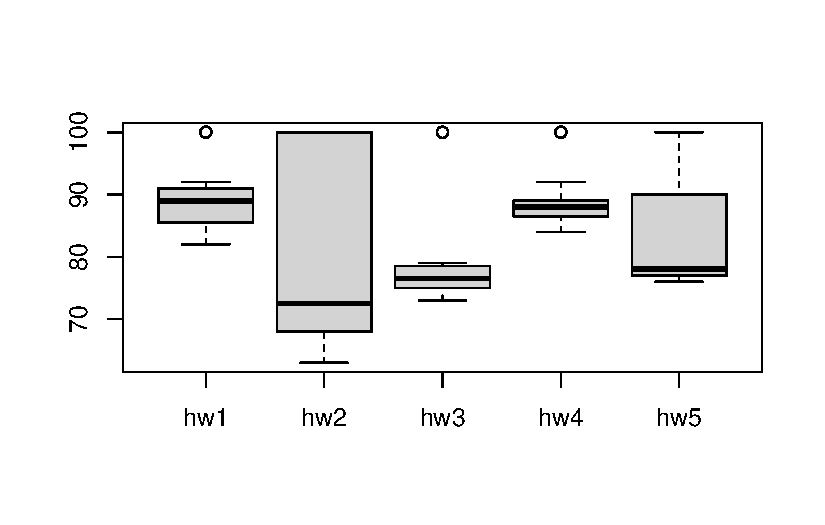
\includegraphics{lab06_files/figure-pdf/unnamed-chunk-10-1.pdf}

}

\end{figure}

\begin{quote}
Q4
\end{quote}

\begin{Shaded}
\begin{Highlighting}[]
\FunctionTok{cor}\NormalTok{(mask}\SpecialCharTok{$}\NormalTok{hw5,results)}
\end{Highlighting}
\end{Shaded}

\begin{verbatim}
[1] 0.6325982
\end{verbatim}

\begin{Shaded}
\begin{Highlighting}[]
\FunctionTok{apply}\NormalTok{(mask, }\DecValTok{2}\NormalTok{, cor, results)}
\end{Highlighting}
\end{Shaded}

\begin{verbatim}
      hw1       hw2       hw3       hw4       hw5 
0.4250204 0.1767780 0.3042561 0.3810884 0.6325982 
\end{verbatim}

\hypertarget{hw6}{%
\subsection{HW6}\label{hw6}}

\begin{Shaded}
\begin{Highlighting}[]
\FunctionTok{library}\NormalTok{(bio3d) }
\NormalTok{prostr }\OtherTok{\textless{}{-}} \ControlFlowTok{function}\NormalTok{(x, }\AttributeTok{chain\_name =} \StringTok{"A"}\NormalTok{, }\AttributeTok{elety\_name =} \StringTok{"CA"}\NormalTok{, }\AttributeTok{yl =} \StringTok{"Bfactor"}\NormalTok{, }\AttributeTok{atom\_col =} \StringTok{"b"}\NormalTok{)\{}
\NormalTok{  s }\OtherTok{\textless{}{-}} \FunctionTok{read.pdb}\NormalTok{(x)}
\NormalTok{  s.chain }\OtherTok{\textless{}{-}} \FunctionTok{trim.pdb}\NormalTok{(s, }\AttributeTok{chain =}\NormalTok{ chain\_name, }\AttributeTok{elety =}\NormalTok{ elety\_name)}
\NormalTok{  s.atom }\OtherTok{\textless{}{-}}\NormalTok{ s.chain}\SpecialCharTok{$}\NormalTok{atom[,atom\_col]}
  \FunctionTok{plotb3}\NormalTok{(s.atom, }\AttributeTok{sse=}\NormalTok{s.chain, }\AttributeTok{typ=}\StringTok{"l"}\NormalTok{, }\AttributeTok{ylab =}\NormalTok{ yl)}
\NormalTok{\}}
\FunctionTok{prostr}\NormalTok{(}\StringTok{"4AKE"}\NormalTok{)}
\end{Highlighting}
\end{Shaded}

\begin{verbatim}
  Note: Accessing on-line PDB file
\end{verbatim}

\begin{figure}[H]

{\centering 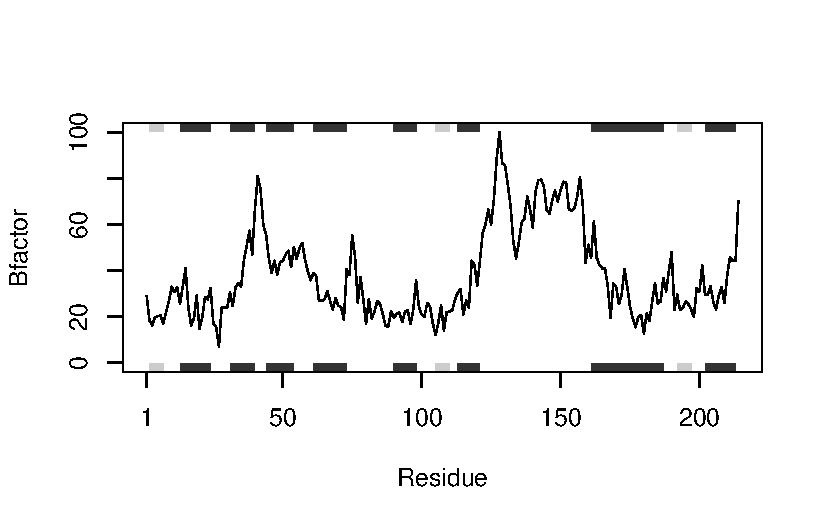
\includegraphics{lab06_files/figure-pdf/unnamed-chunk-14-1.pdf}

}

\end{figure}



\end{document}
